\documentclass{article}
\usepackage{setspace}
\usepackage[text={6.5in,8.5in},centering]{geometry}
\geometry{verbose,a4paper,tmargin=2.4cm,bmargin=2.4cm,lmargin=2.4cm,rmargin=2.4cm}
\usepackage{graphicx,amsmath,cases,multirow,appendix,graphicx,xcolor,cancel,tikz}

\setlength\parindent{0pt}

\newcommand{\note}[1]{\colorbox{gray!30}{#1}}
\newcommand{\ind}{\-\hspace{1cm}}
\newcommand*\circled[1]{\tikz[baseline=(char.base)]{
            \node[shape=circle,draw,inner sep=2pt] (char) {#1};}}


\begin{document}

\noindent\makebox[\textwidth][c]{\Large\bfseries Lecture 6 -- Model-fitting - observation \& process error}

\rule[0.5ex]{\linewidth}{1pt}
\textbf{Announcements}:\\
Finish up MSY first ($\sim$ 20 min.) \& collect Q2\\
Next time: Maximum Likelihood, AIC, \& Paper discussion

\textbf{Concepts}: \\
Process vs. Observation error

\rule[0.5ex]{\linewidth}{1pt}
\textbf{Types of Error}\\
\emph{Process error}\\
\ind Environmental stochasticity\\
\ind Demographic stochasticity\\
\ind \ind ...both include biotic (intra \& interspecific intxns.) and abiotic effects on vital rates.\\
\emph{Observation error} (aka Measurement error)\\
\ind Variation due to observers (e.g., bias: experienced vs. novice observer)\\
\ind Sample estimation (only subset of total observed)\\

Implications of attributing error:
\begin{center}
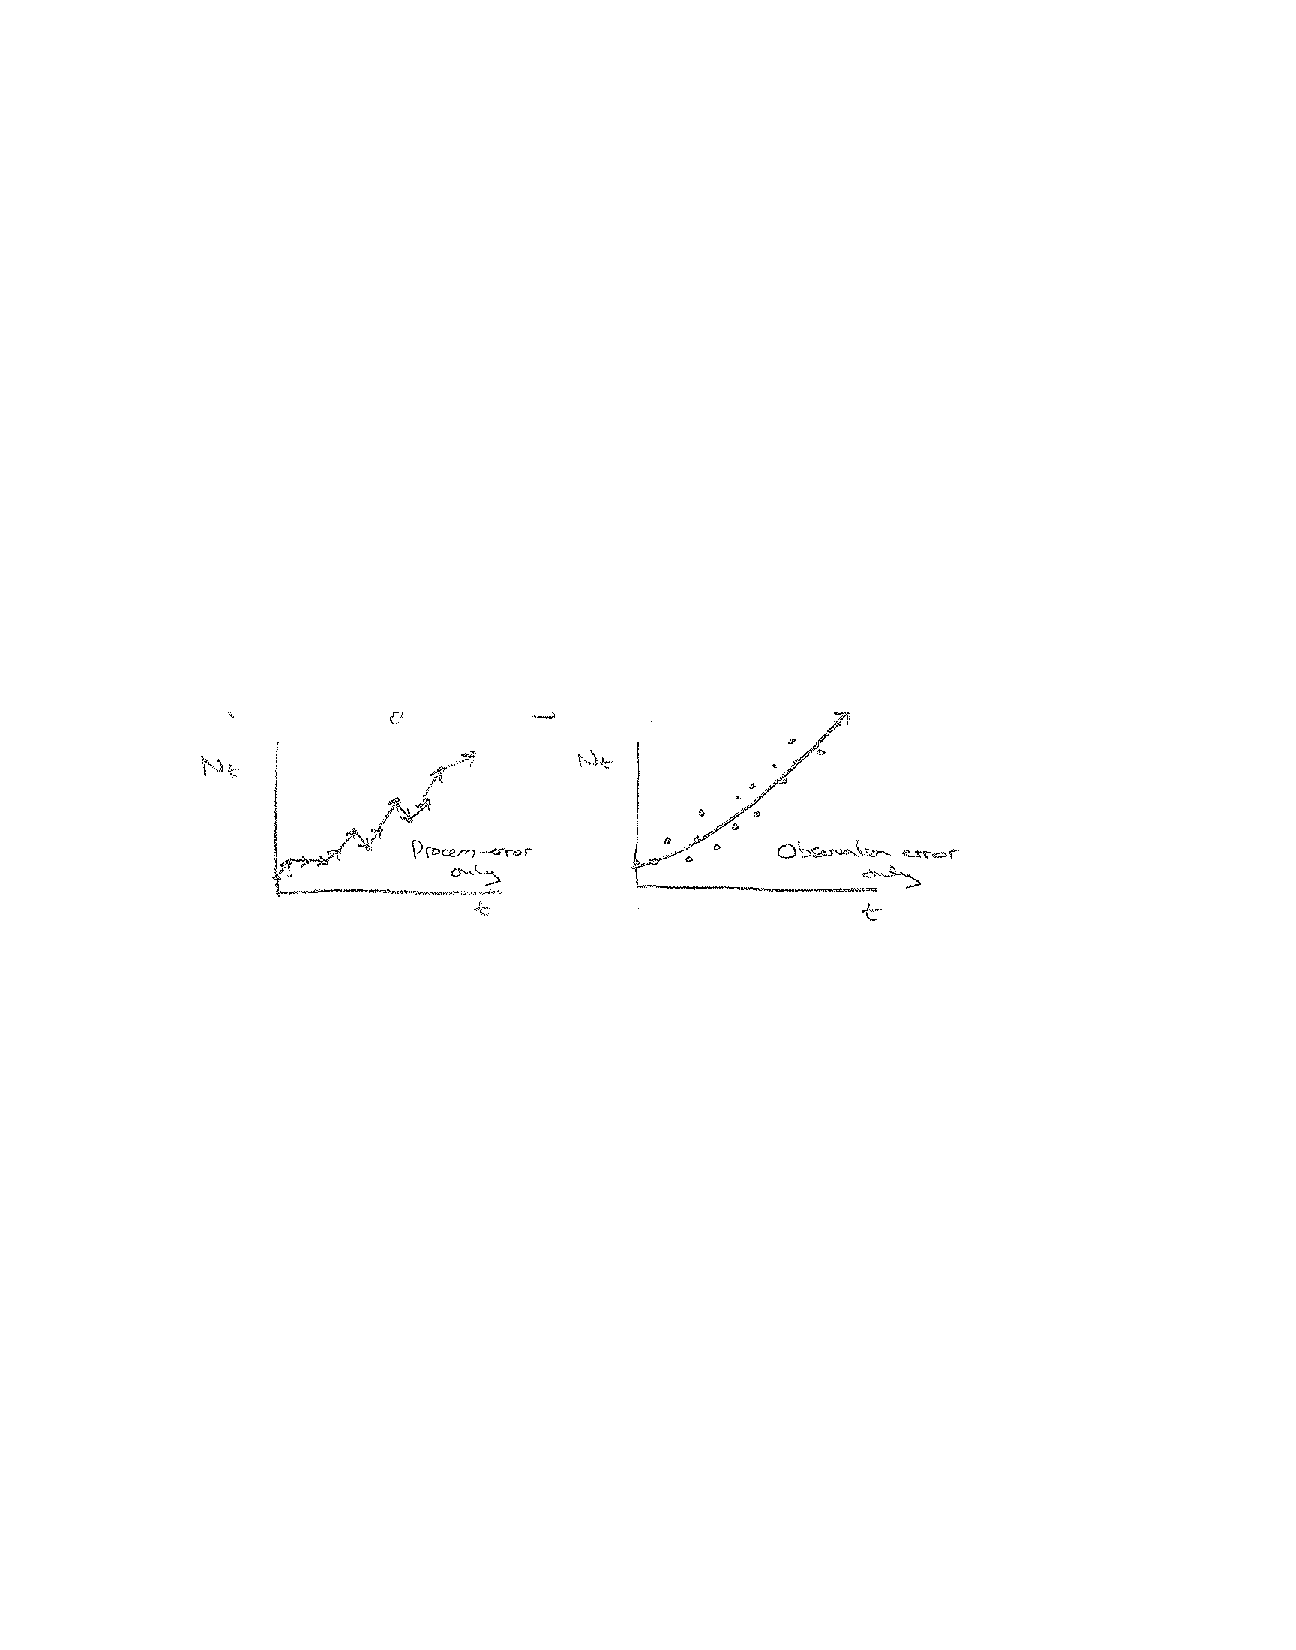
\includegraphics[width=10cm]{figs/image0.pdf}
\end{center}
\rule[0.5ex]{\linewidth}{1pt}

\textbf{Estimation of Observation error}\\
``Trajectory matching'': 
Calculate standard deviations of ``expected'' trajectory given hypothesized model and expected distribution of residuals.

\begin{center}
	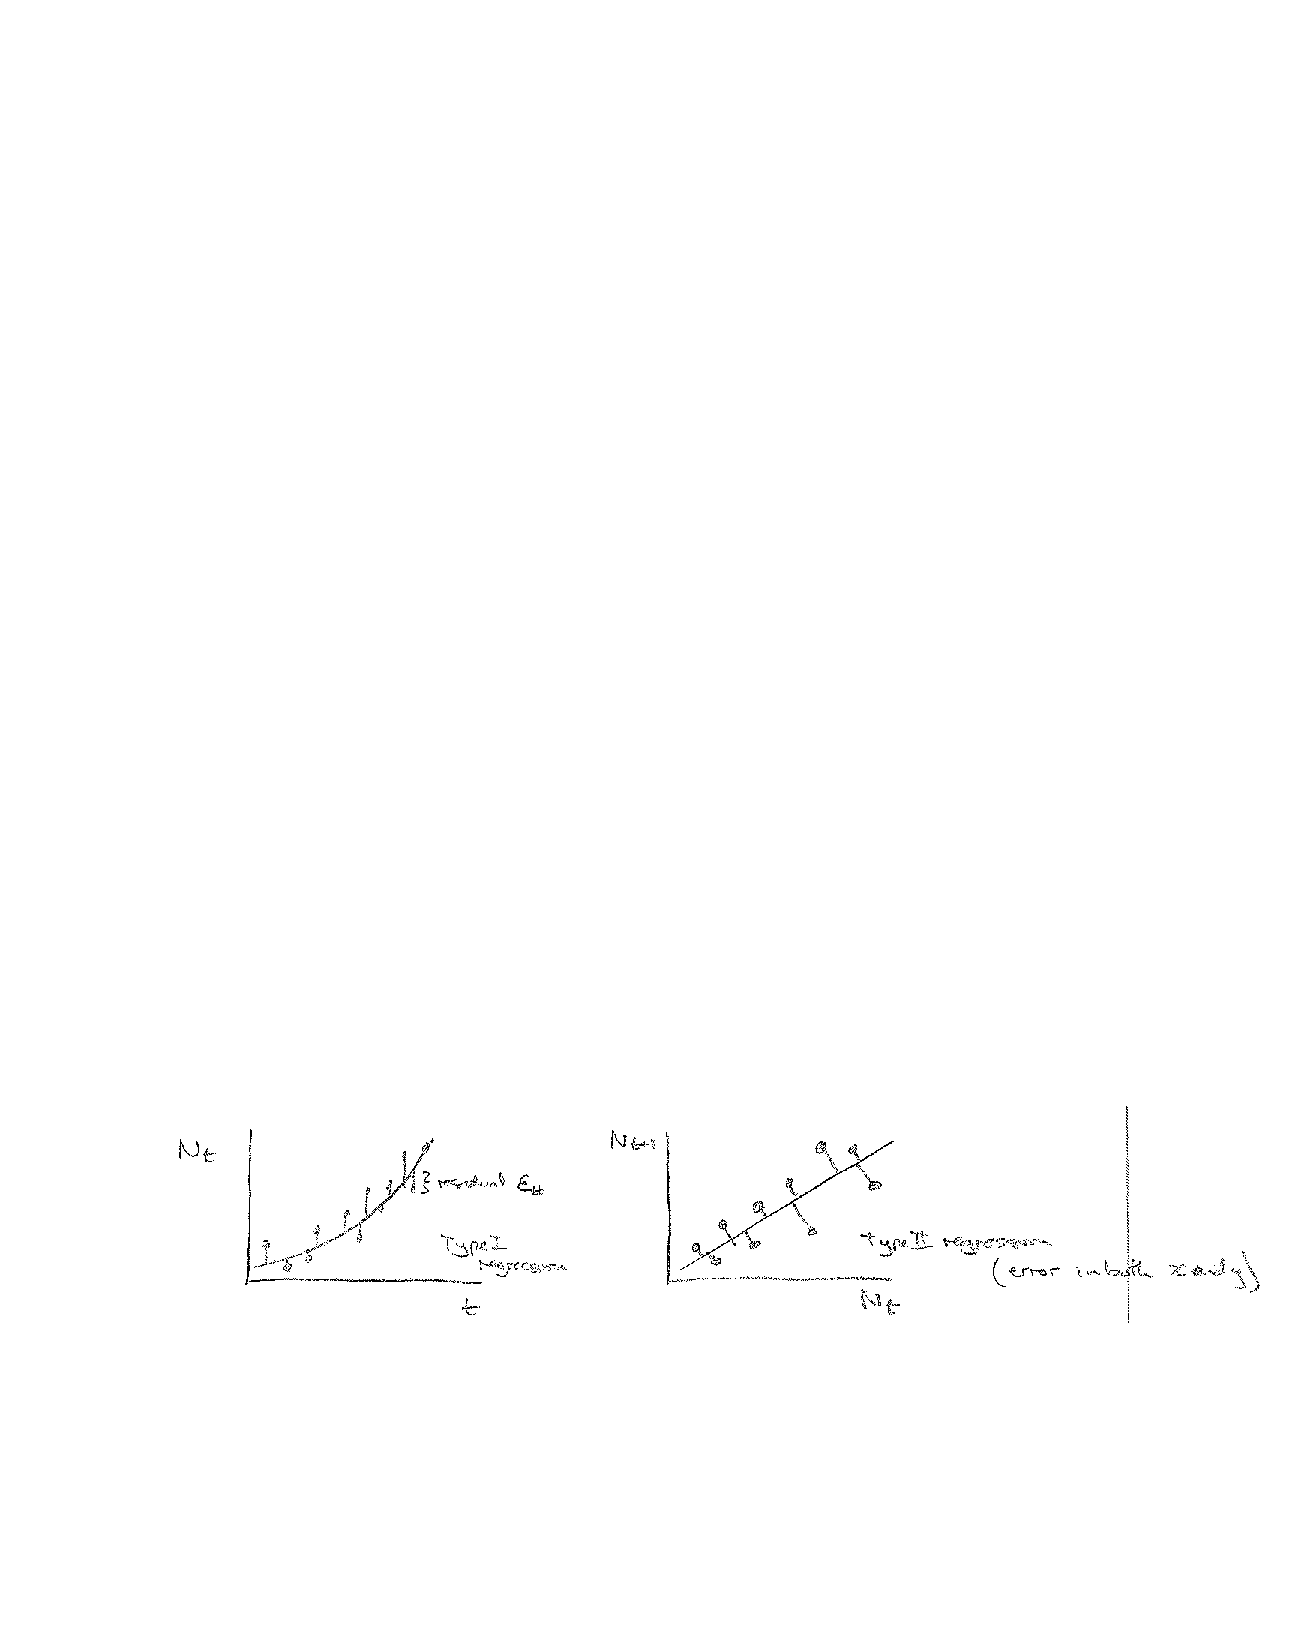
\includegraphics[width=12cm]{figs/image1.pdf}
\end{center}

Estimate ``best'' model parameters using:\\
\ind - Least-squares regression (Type I or Type II) if $\epsilon \sim \mathcal{N}(\mu, \sigma)$\\
\ind - Maximum likelihood \emph{will explain later}\\
\ind \ind \ind (equivalent to least-squares if $\epsilon \sim \mathcal{N}(\mu, \sigma)$)\\

E.g., Type I regression:\\
\begin{align*}
	N_t &= N_0 e^{rt}\\
	log(N_t) & = log(N_0)+rt \quad \quad &\text{``Deterministic/Process model''} \quad \quad  &\Rightarrow y=a + bx\\
	\\
	log(N_t) & = log(N_0)+rt+\epsilon \quad \quad &\text{``Stochastic/Statistical model''} \quad \quad &\Rightarrow y=a + bx + \epsilon \\
	\epsilon &\sim iid \mathcal{N}(\mu,\sigma)
\end{align*}

Residual at point $t$: $\quad \epsilon_t = \log N_{obs,t} - \log N_{pred,t}$\\

``Best'' least-squares parameter estimates (i.e.\emph{``most likely given the data.''})\\
\ind are at $\mu = 0$ and $\sum\epsilon^2 = \min{\sum\epsilon^2}$ (i.e. \emph{least} squares).\\

MLE's for slope and intercept (using $\hat{x}$ to indicate estimate):
\begin{align*}
	\hat{b} &= \rho_{xy}\frac{\sigma^2_y}{\sigma^2_x} \quad \text{where } \rho_{xy} \text{ is the Pearson correlation coefficient} \quad &\Rightarrow \hat{r} = \rho_{\log N_t,t}\frac{ \sigma^2_{\log N_t}}{\sigma^2_t}\\
	\hat{a} &= \bar{y}-\hat{b}\bar{x} &\Rightarrow \widehat{log(N_0)} = \bar{\log N_t} - \hat{r} \bar{t}
\end{align*}

Note, for series of $n$ observations of $N$:
\begin{equation*}
\text{Observer error } = \hat{\sigma}_{obs}^2 = \underbrace{\frac{1}{n-1}}_{\substack{\text{small sample}\\ \text{correction}}} \sum_t^n\left(log(N_{t,obs}) - log(N_{t,pred})\right)^2
\end{equation*}

\rule[0.5ex]{\linewidth}{1pt}

\textbf{Estimating Process Error}
\begin{center}
	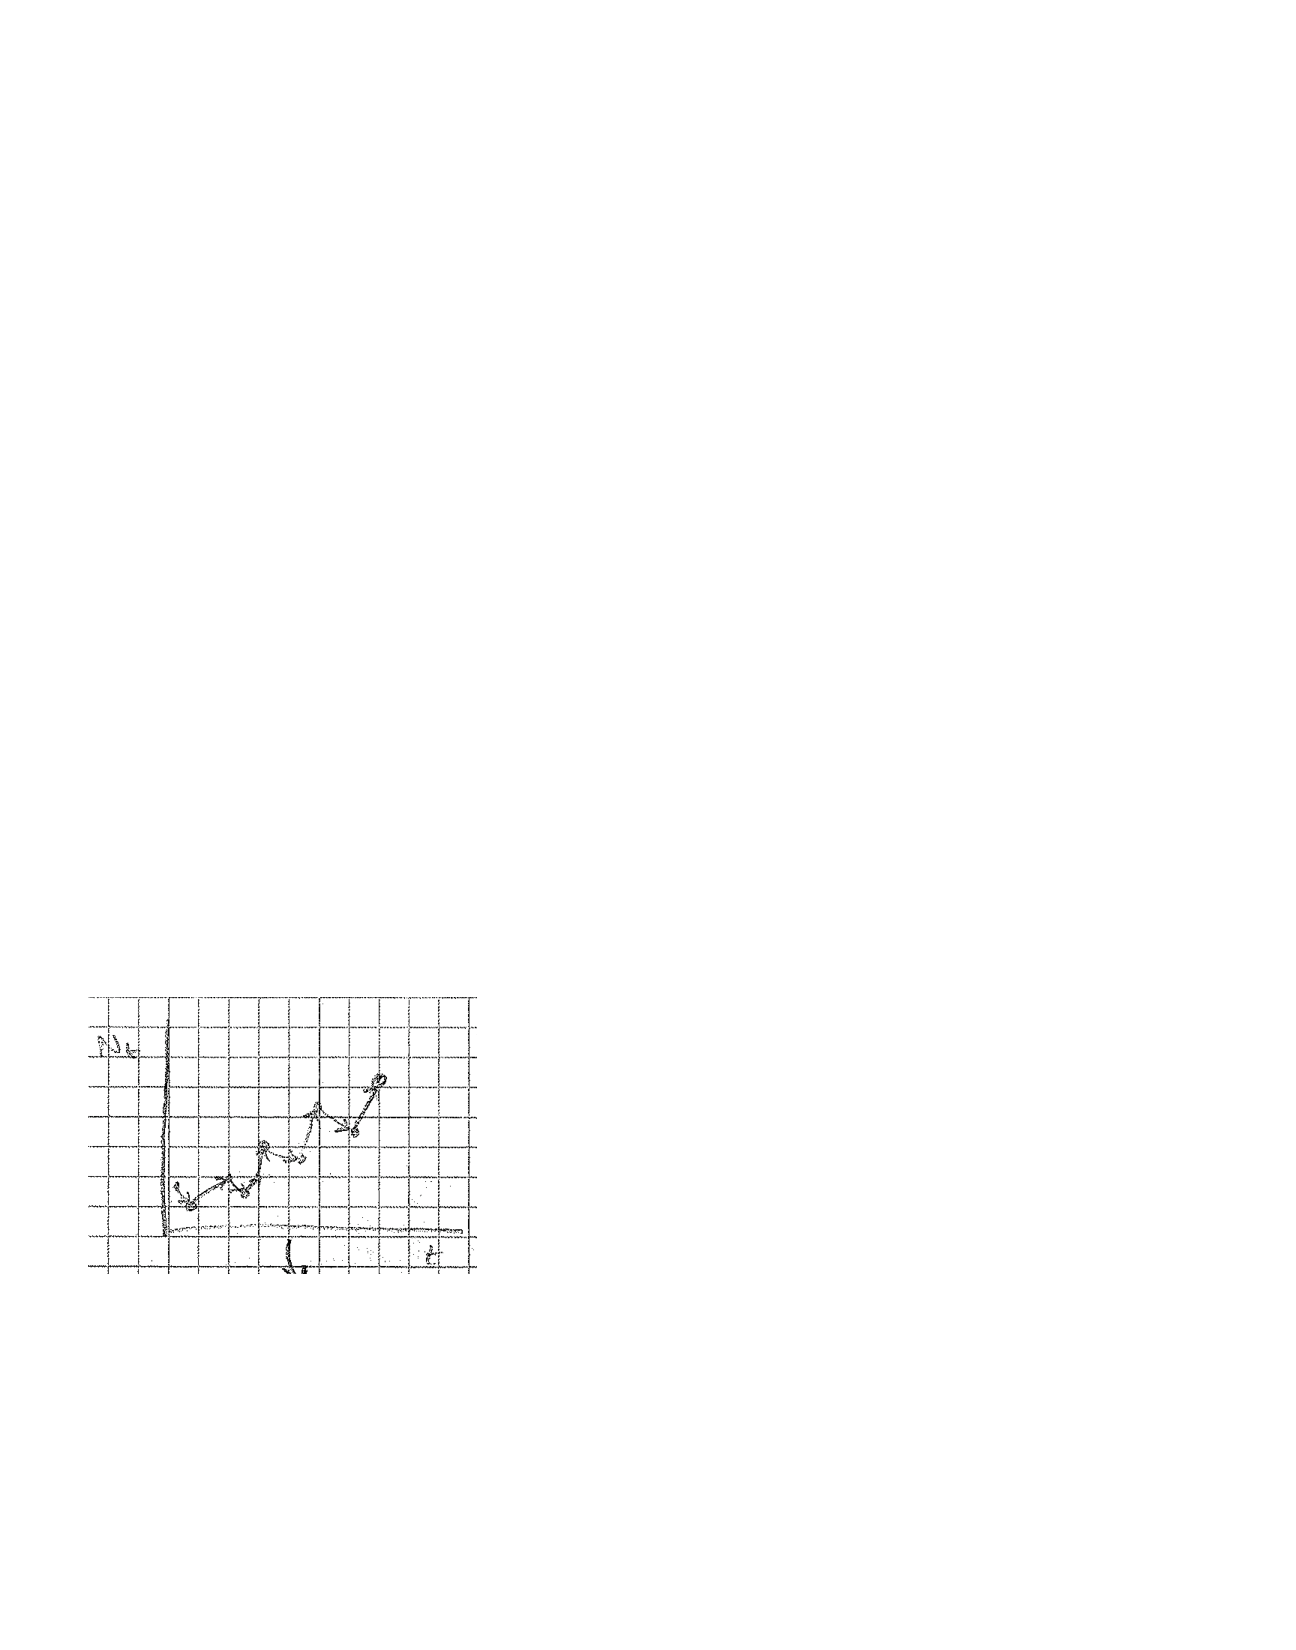
\includegraphics[width=5cm]{figs/image2a.pdf}
	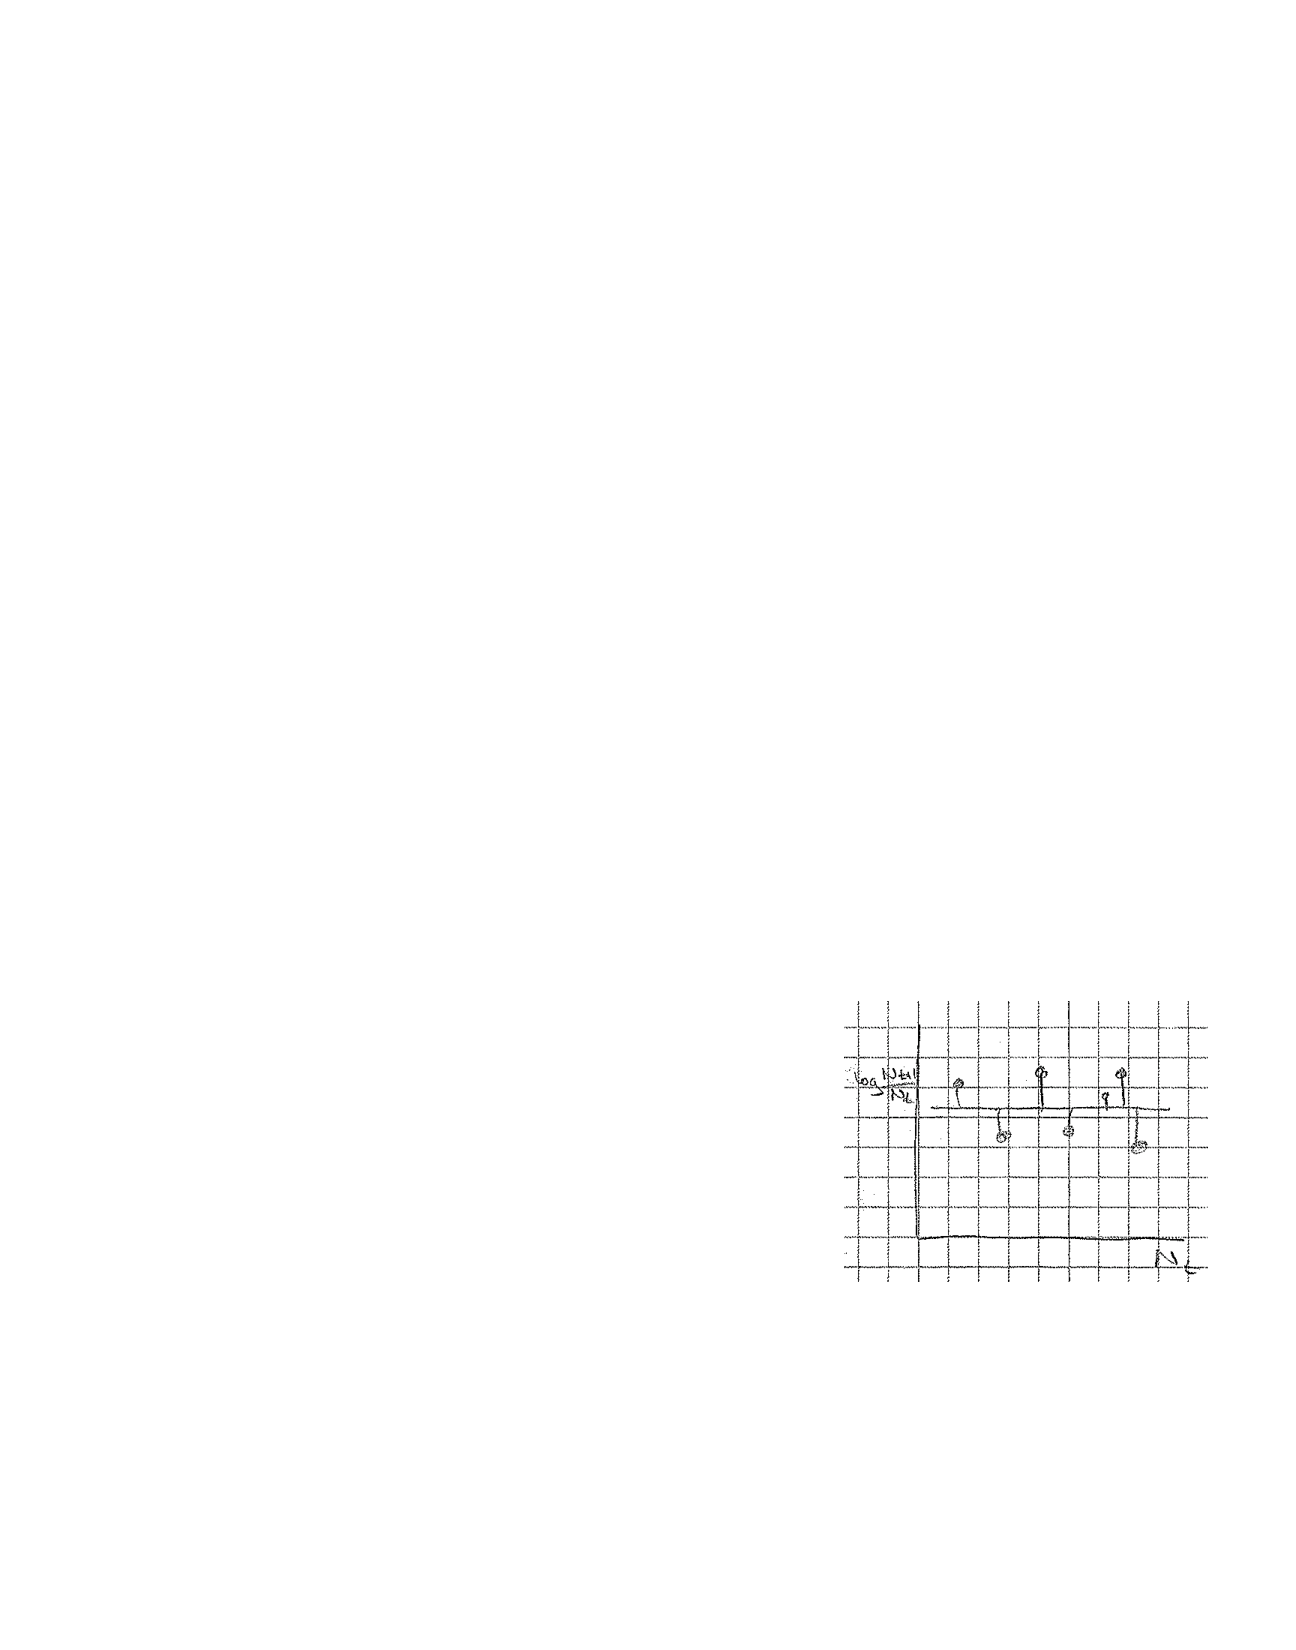
\includegraphics[width=5cm]{figs/image2b.pdf}
\end{center}
``One step-ahead'' prediction\\
\ind Estimating error of process at each time-step.\\
\ind \ind ``Process'' = growth rate\\

Step 1: Calculate log-transformed growth rates from data:\\
\begin{equation*}
	\ln \left(\frac{N_{t+1}}{N_t}\right) \quad \quad \text{or} \quad \quad 	\ln\left(\frac{N_{t+\Delta t}}{N_t}\right) \bigg / \Delta t
\end{equation*}

Step 2: Specify hypothesized process model, and rearrange to solve for $\ln \left(\frac{N_{t+1}}{N_t}\right)$\\
\ind e.g., for density-independent growth:\\
\begin{equation*}
	\ln\left(\frac{N_{t+1}}{N_t}\right) = \ln\left(\frac{F(N_t)}{N_t}\right) = \ln\left(\frac{\lambda N_t}{N_t}\right) = \ln \lambda = \ln (e^r) = r
\end{equation*}

Step 3: Specify statistical model and fit to data (LS or MaxLik, etc.):
\begin{center}
	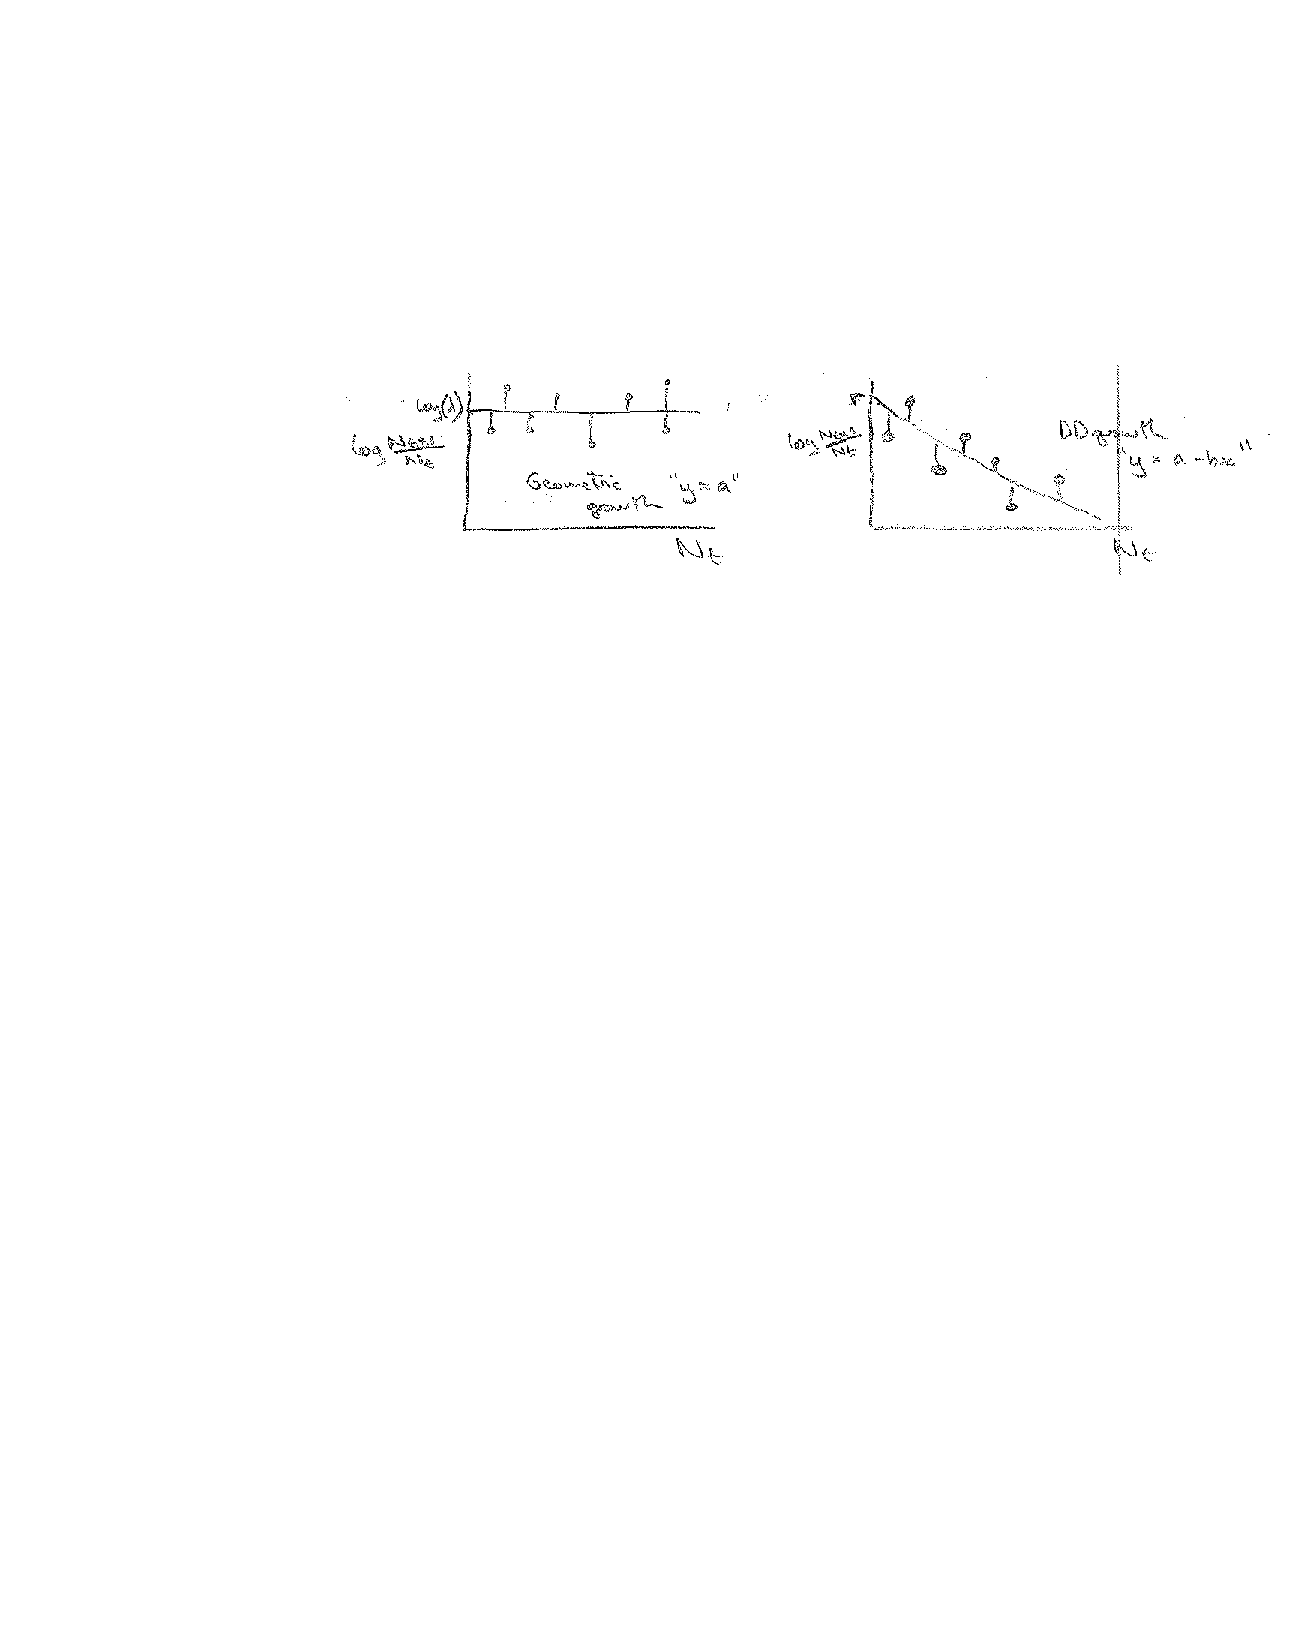
\includegraphics[width=15cm]{figs/image3.pdf}
\end{center}

Estimated process error:
\begin{equation*}
	\hat{\sigma}_{est}^2 = \frac{1}{n-1}\sum \left(\ln\left(\frac{N_{t+1}}{N_t}\right)_{obs} - \ln\left(\frac{N_{t+1}}{N_t}\right)_{pred}\right)^2
\end{equation*}

\rule[0.5ex]{\linewidth}{1pt}

\pagebreak
\note{R exercise} - Load \emph{Class-6.R} and data (SAFseal1, Grizzlies, Redsword)\\
\ind \note{Walk through code}\\
\ind \ind - observation error\\
\ind \ind - process error\\
\ind \ind - forecast w/ process error vs. observation error\\

Observation error:
\begin{align*}
	N_t=N_0 e^{rt} \quad \Rightarrow \quad \ln{N_t}=\ln{N_0}+rt+\epsilon_t \\
	\note{ in R: $lm(y\sim x)$}
\end{align*}

Process error:
\begin{align*}
	\ln\left(\frac{N_{t+1}}{N_t}\right) = r + \epsilon_t \quad \quad = \beta_0 + \cancelto{0}{\beta_1} N_t + \epsilon_t \quad \text{for density-independence}\\
	\note{ in R: $lm(y\sim 1)$ or just $mean$()!}
\end{align*}
\ind In words, the best estimate for $\hat{r}$ is the mean of all $\log \left(\frac{N_{t+1}}{N_t}\right)_t$

\rule[0.5ex]{\linewidth}{1pt}
\textbf{What if both types!?!}\\
Ignoring observation error will inflate process error.\\
Standard methods can't disentangle them.\\
\ind (Rule of thumb is that you're okay if observation error is $<10\%$ of values.)\\

Most common solutions:\\

\circled{1} Use independent estimates (replicate surveys of same population)\\
Let $\hat{N_t} = \frac{1}{n}\sum_i^n N_{t,i}$ for $n$ independent surveys at time $t$.\\
\ind Then $\hat{N}$ is nearly unbiased estimator of true $N$.\\
For process error:\\
\ind Use $\hat{N}$ to calculate $\ln\left(\frac{\hat{N}_{t+1}}{\hat{N}_t}\right)$ and proceed to estimate $\sigma_{proc}^2$ (see Morris \& Doak eqn. 5.5).\\
For observation error:\\
\begin{equation*}
	\sigma_{obs}^2 = \frac{1}{n-1}\sum_i^n \left(N_{t,i}-\hat{N}_t\right)^2
\end{equation*}

\circled{2} State-space models\\
Combine process- w/ observation model:
\begin{center}
	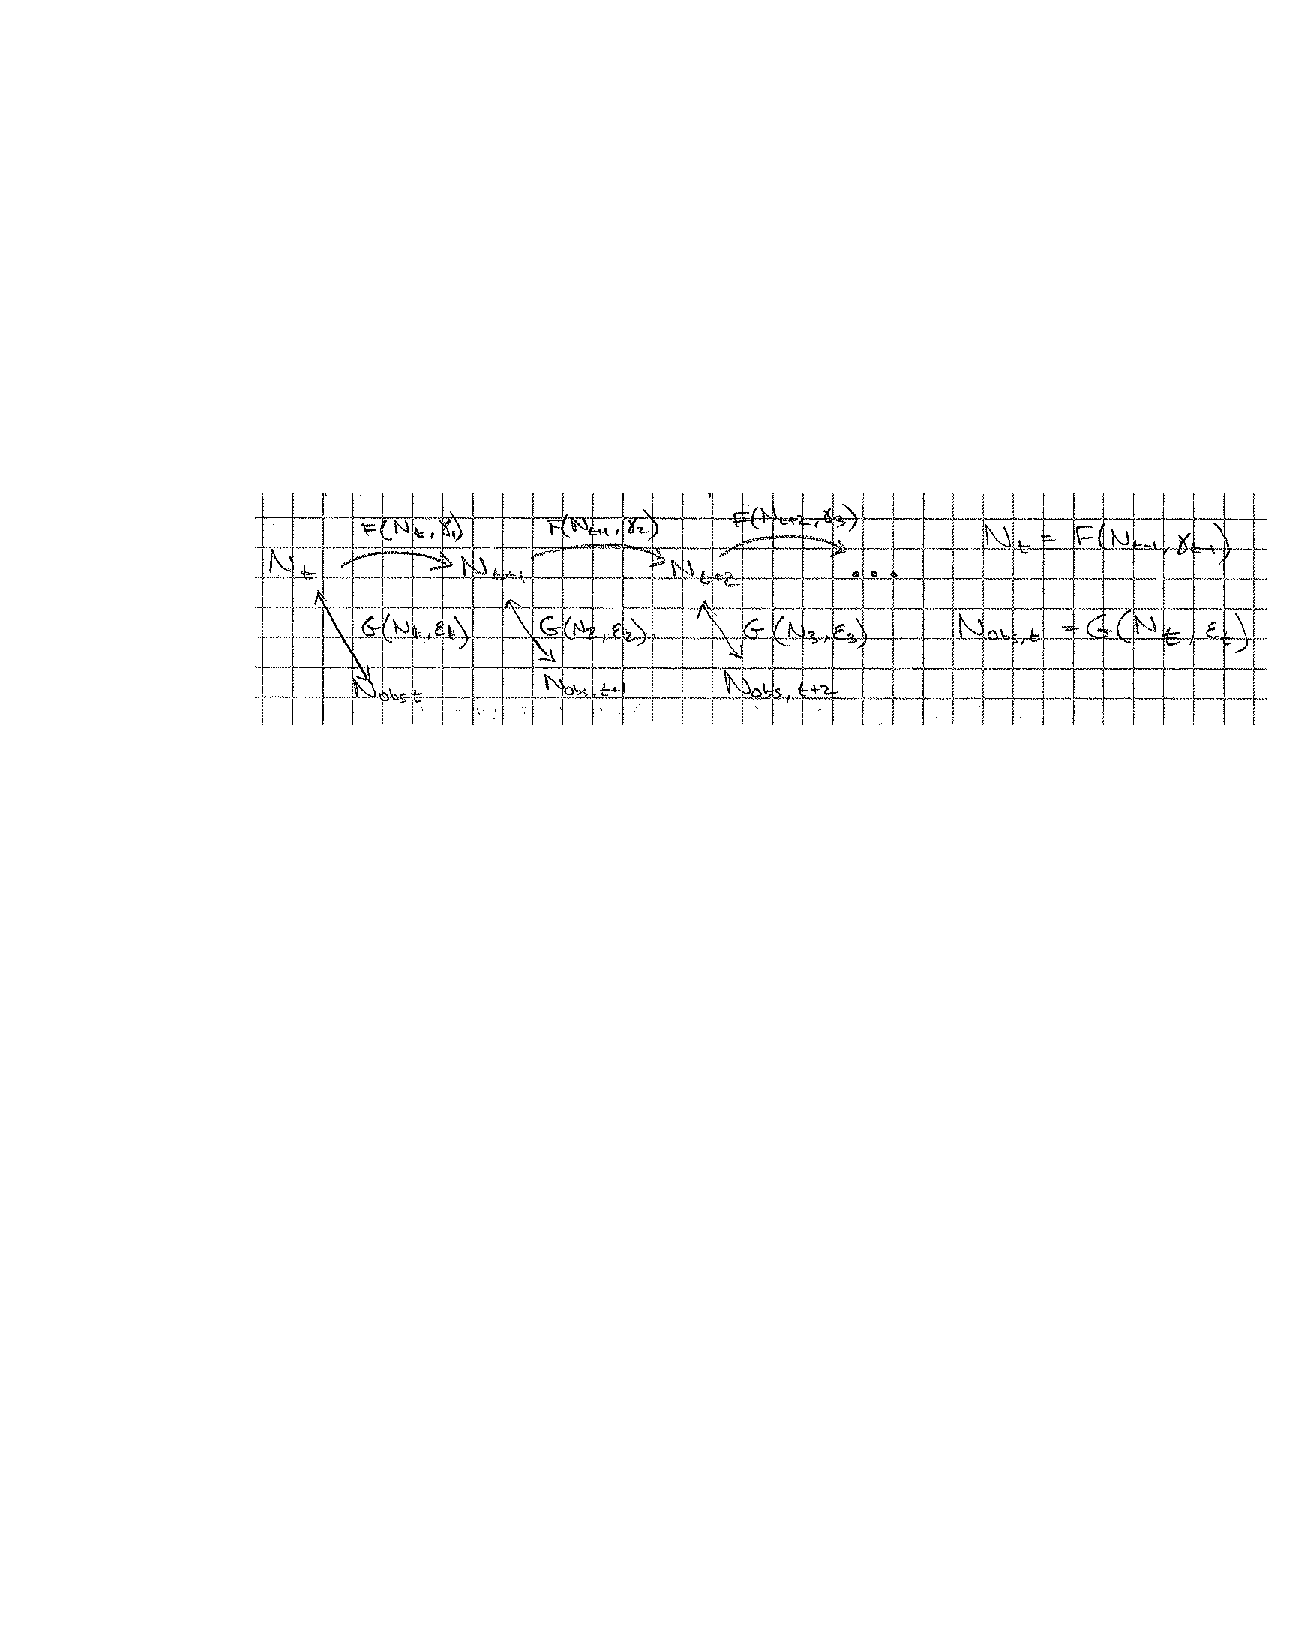
\includegraphics[width=16cm]{figs/image4.pdf}
\end{center}

Methods include Maximum likelihood \& Bayesian, using Kalman filters, etc.\\
\ind ...disentangle $\gamma$ from $\epsilon$ assuming specified distributions for these.

\rule[0.5ex]{\linewidth}{1pt}
\rule[0.5ex]{\linewidth}{1pt}

\end{document}